% =====================================================================
%  SIC 8 · Big Data Engineering · Project 03 — Project Proposal (2 pages)
%  Compile on Overleaf with pdfLaTeX (default). No external images needed.
% =====================================================================
\documentclass[10pt,a4paper]{article}

\usepackage[a4paper,top=11mm,bottom=13mm,left=12mm,right=12mm,footskip=6mm]{geometry}
\usepackage[T1]{fontenc}
\usepackage[utf8]{inputenc}
\usepackage[scaled=0.95]{helvet}
\renewcommand{\familydefault}{\sfdefault}
\usepackage{microtype}
\usepackage[table]{xcolor}
\usepackage{tikz}
\usetikzlibrary{arrows.meta,positioning,fit,backgrounds}
\usepackage{tabularx}
\usepackage{array}
\usepackage{booktabs}
\usepackage{enumitem}
\usepackage[most]{tcolorbox}
\usepackage{titlesec}
\usepackage{fancyhdr}
\usepackage{amssymb}
\usepackage{textcomp}

% ---------- colours ----------
\definecolor{navy}{HTML}{0B1560}
\definecolor{blue}{HTML}{1428A0}
\definecolor{aws}{HTML}{C2410C}
\definecolor{snow}{HTML}{0E7490}
\definecolor{gray7}{HTML}{374151}
\definecolor{ink}{HTML}{1F2937}
\definecolor{muted}{HTML}{4B5563}
\definecolor{lightblue}{HTML}{EEF2FF}
\definecolor{rowalt}{HTML}{F8FAFF}
\definecolor{snowbg}{HTML}{E6F4F6}
\definecolor{cardline}{HTML}{C7D2FE}

\color{ink}
\setlength{\parindent}{0pt}
\setlength{\parskip}{2pt}
\linespread{1.02}

% ---------- headings ----------
\titleformat{\section}{\color{navy}\bfseries\normalsize}{}{0pt}{}[\vspace{-6pt}{\color{blue}\rule{\linewidth}{1.2pt}}]
\titlespacing*{\section}{0pt}{7pt}{1pt}

% ---------- footer ----------
\pagestyle{fancy}
\fancyhf{}
\renewcommand{\headrulewidth}{0pt}
\fancyfoot[L]{\tiny\color{muted} SIC 8 · Project 03 · Fleet Telematics Lakehouse · Proposal}
\fancyfoot[R]{\tiny\color{muted}\thepage\ / 2}

% ---------- helpers ----------
\newcommand{\code}[1]{\colorbox{lightblue}{\ttfamily\scriptsize #1}}
\newtcolorbox{card}[1]{enhanced, colback=white, colframe=cardline, boxrule=0.6pt, arc=3pt,
  left=4pt, right=4pt, top=3pt, bottom=3pt, fontupper=\footnotesize,
  before upper={{\small\bfseries\color{navy}#1\par}\vspace{2pt}}}
\setlist[itemize]{leftmargin=9pt, itemsep=1pt, topsep=1pt, parsep=0pt, label=\textbullet}
\newcolumntype{Y}{>{\raggedright\arraybackslash}X}
\newcommand{\thead}[1]{\textcolor{white}{\bfseries #1}}
\renewcommand{\arraystretch}{1.18}

% table header row colour
\newcommand{\ttl}{\footnotesize\bfseries}
\newcommand{\headrow}{\rowcolor{navy}}

\begin{document}

% =====================================================================
%  PAGE 1
% =====================================================================
{\color{blue}\scriptsize\bfseries SIC 8 \textperiodcentered{} BIG DATA ENGINEERING \textperiodcentered{} PROJECT 03 \textperiodcentered{} PROJECT PROPOSAL}\\[1pt]
{\raggedright\hyphenpenalty=10000\color{navy}\Large\bfseries Enterprise Fleet Telematics Lakehouse \& Dynamic Logistics Warehouse\par}\vspace{2pt}
{\scriptsize\color{muted} Team of 3 · 6 build days · Hybrid delivery: local Docker (generator, Kafka, Airbyte, Airflow, FastAPI, React) + cloud (Amazon S3, Snowflake)}

\vspace{4pt}
\begin{tcbraster}[raster columns=3, raster equal height, raster column skip=6pt, colback=white, colframe=cardline, boxrule=0.6pt, arc=3pt, left=4pt, right=4pt, top=3pt, bottom=3pt, fontupper=\footnotesize\raggedright]
\begin{tcolorbox}
{\small\bfseries\color{navy}Problem\par}\vspace{2pt}
Fleet managers cannot combine vehicle diagnostics, position and cargo temperature in one place, so route deviations, refrigeration breaches and excessive idling are hard to investigate consistently.
\end{tcolorbox}
\begin{tcolorbox}
{\small\bfseries\color{navy}Objective\par}\vspace{2pt}
Build a telematics lakehouse and star-schema warehouse for \textbf{5,000 simulated delivery vehicles} on fixed corridors, serving route fuel efficiency, cold-chain compliance \% and driver safety/idling scorecards in a 3D web dashboard.
\end{tcolorbox}
\begin{tcolorbox}
{\small\bfseries\color{navy}Measurable targets\par}\vspace{2pt}
5,000 distinct vehicles · 0 duplicate keys in silver · Kafka = S3 = RAW + load errors · detection recall $\geq$ 95\% / precision $\geq$ 90\% vs injected truth · dashboard = API = SQL $\pm$0.1\% · event $\rightarrow$ KPI $\leq$ 15 min.
\end{tcolorbox}
\end{tcbraster}

\section{End-to-end flow}

\begin{tcolorbox}[enhanced, colback=white, colframe=gray!25, boxrule=0.5pt, arc=3pt, left=2pt, right=2pt, top=2pt, bottom=2pt]
\centering
\resizebox{\linewidth}{!}{%
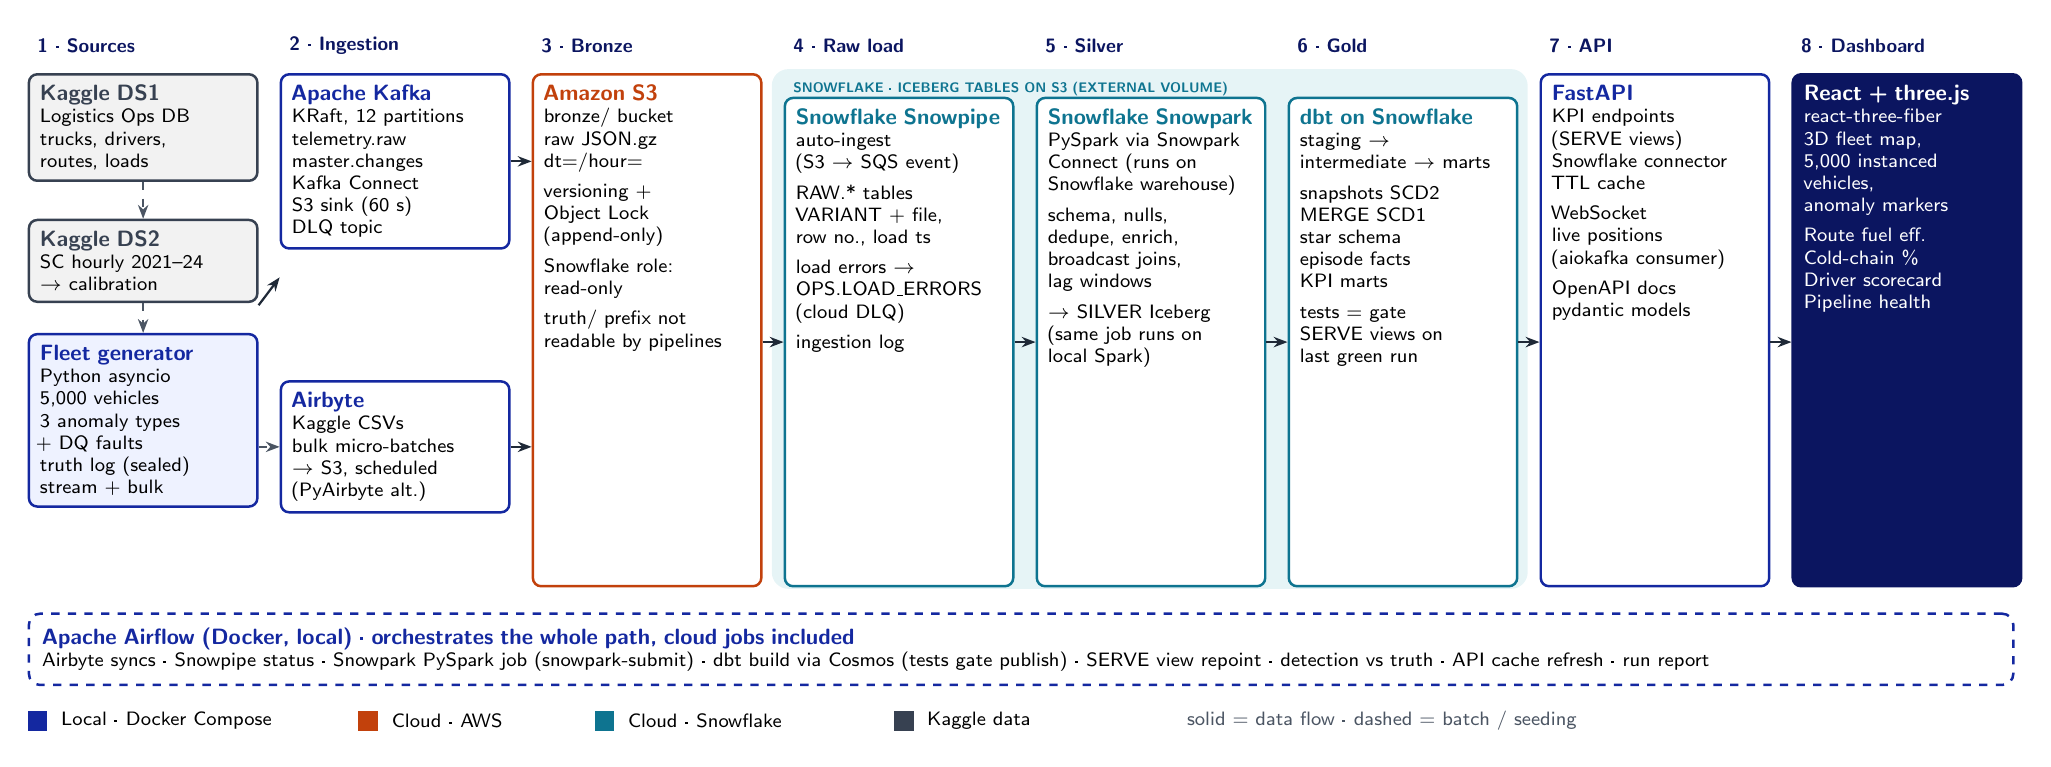
\begin{tikzpicture}[
  font=\sffamily,
  box/.style={draw=#1, line width=0.9pt, rounded corners=3pt, fill=white, align=left,
              anchor=north west, text width=2.62cm, inner sep=4pt, font=\scriptsize\sffamily},
  hd/.style={font=\scriptsize\bfseries\sffamily, text=navy, anchor=west},
  flow/.style={-{Stealth[length=5pt]}, line width=0.8pt, draw=ink},
  dflow/.style={-{Stealth[length=5pt]}, line width=0.8pt, draw=muted, dashed},
]
% column x positions (cm)
\def\cA{0}  \def\cB{3.2} \def\cC{6.4} \def\cD{9.6}
\def\cE{12.8} \def\cF{16.0} \def\cG{19.2} \def\cH{22.4}

% headers
\node[hd] at (\cA,0.35) {1 · Sources};
\node[hd] at (\cB,0.35) {2 · Ingestion};
\node[hd] at (\cC,0.35) {3 · Bronze};
\node[hd] at (\cD,0.35) {4 · Raw load};
\node[hd] at (\cE,0.35) {5 · Silver};
\node[hd] at (\cF,0.35) {6 · Gold};
\node[hd] at (\cG,0.35) {7 · API};
\node[hd] at (\cH,0.35) {8 · Dashboard};

% Snowflake region
\fill[snowbg, rounded corners=6pt] (\cD-0.15,0.05) rectangle (\cF+3.05,-6.55);
\node[anchor=west, font=\tiny\bfseries\sffamily, text=snow] at (\cD,-0.2) {SNOWFLAKE · ICEBERG TABLES ON S3 (EXTERNAL VOLUME)};

% sources
\node[box=gray7, fill=gray!10] (ds1) at (\cA,0) {{\ttl\color{gray7} Kaggle DS1}\\Logistics Ops DB\\trucks, drivers,\\routes, loads};
\node[box=gray7, fill=gray!10] (ds2) at (\cA,-1.85) {{\ttl\color{gray7} Kaggle DS2}\\SC hourly 2021--24\\$\rightarrow$ calibration};
\node[box=blue, fill=lightblue] (gen) at (\cA,-3.3) {{\ttl\color{blue} Fleet generator}\\Python asyncio\\5,000 vehicles\\3 anomaly types\\+ DQ faults\\truth log (sealed)\\stream + bulk};
\draw[dflow] (ds1.south) -- (ds2.north);
\draw[dflow] (ds2.south) -- (gen.north);

% ingestion
\node[box=blue] (kafka) at (\cB,0) {{\ttl\color{blue} Apache Kafka}\\KRaft, 12 partitions\\telemetry.raw\\master.changes\\Kafka Connect\\S3 sink (60 s)\\DLQ topic};
\node[box=blue] (airbyte) at (\cB,-3.9) {{\ttl\color{blue} Airbyte}\\Kaggle CSVs\\bulk micro-batches\\$\rightarrow$ S3, scheduled\\(PyAirbyte alt.)};

% bronze
\node[box=aws] (s3) at (\cC,0) {\parbox[t][6.22cm][t]{2.62cm}{\raggedright {\ttl\color{aws} Amazon S3}\\bronze/ bucket\\raw JSON.gz\\dt=/hour=\\[3pt]versioning +\\Object Lock\\(append-only)\\[3pt]Snowflake role:\\read-only\\[3pt]truth/ prefix not\\readable by pipelines}};

% snowflake columns
\node[box=snow] (pipe) at (\cD,-0.3) {\parbox[t][5.92cm][t]{2.62cm}{\raggedright {\ttl\color{snow} Snowflake Snowpipe}\\auto-ingest\\(S3 $\rightarrow$ SQS event)\\[3pt]RAW.* tables\\VARIANT + file,\\row no., load ts\\[3pt]load errors $\rightarrow$\\OPS.LOAD\_ERRORS\\(cloud DLQ)\\[3pt]ingestion log}};
\node[box=snow] (spark) at (\cE,-0.3) {\parbox[t][5.92cm][t]{2.62cm}{\raggedright {\ttl\color{snow} Snowflake Snowpark}\\PySpark via Snowpark\\Connect (runs on\\Snowflake warehouse)\\[3pt]schema, nulls,\\dedupe, enrich,\\broadcast joins,\\lag windows\\[3pt]$\rightarrow$ SILVER Iceberg\\(same job runs on\\local Spark)}};
\node[box=snow] (dbt) at (\cF,-0.3) {\parbox[t][5.92cm][t]{2.62cm}{\raggedright {\ttl\color{snow} dbt on Snowflake}\\staging $\rightarrow$\\intermediate $\rightarrow$ marts\\[3pt]snapshots SCD2\\MERGE SCD1\\star schema\\episode facts\\KPI marts\\[3pt]tests = gate\\SERVE views on\\last green run}};

% api + dashboard
\node[box=blue] (api) at (\cG,0) {\parbox[t][6.22cm][t]{2.62cm}{\raggedright {\ttl\color{blue} FastAPI}\\KPI endpoints\\(SERVE views)\\Snowflake connector\\TTL cache\\[3pt]WebSocket\\live positions\\(aiokafka consumer)\\[3pt]OpenAPI docs\\pydantic models}};
\node[box=navy, fill=navy, text=white] (web) at (\cH,0) {\parbox[t][6.22cm][t]{2.62cm}{\raggedright {\ttl React + three.js}\\react-three-fiber\\3D fleet map,\\5,000 instanced\\vehicles,\\anomaly markers\\[3pt]Route fuel eff.\\Cold-chain \%\\Driver scorecard\\Pipeline health}};

% flows
\draw[flow] ([yshift=10pt]gen.north east) -- ([yshift=-10pt]kafka.south west);
\draw[dflow] (gen.east|-airbyte.east) -- (airbyte.east-|airbyte.west);
\draw[flow] (kafka.east) -- (s3.west|-kafka.east);
\draw[flow] (airbyte.east) -- (s3.west|-airbyte.east);
\draw[flow] (s3.east|-pipe.center) -- (pipe.west|-pipe.center);
\draw[flow] (pipe.east) -- (spark.west);
\draw[flow] (spark.east) -- (dbt.west);
\draw[flow] (dbt.east) -- (api.west|-dbt.east);
\draw[flow] (api.east|-dbt.east) -- (web.west|-dbt.east);

% Airflow bar
\node[draw=blue, dashed, line width=0.9pt, rounded corners=4pt, anchor=north west,
      text width=24.85cm, inner sep=5pt, align=left, font=\scriptsize\sffamily] at (\cA,-6.85)
  {{\footnotesize\bfseries\color{blue} Apache Airflow (Docker, local) · orchestrates the whole path, cloud jobs included}\\
   Airbyte syncs · Snowpipe status · Snowpark PySpark job (snowpark-submit) · dbt build via Cosmos (tests gate publish) · SERVE view repoint · detection vs truth · API cache refresh · run report};

% legend
\begin{scope}[font=\scriptsize\sffamily]
\fill[blue] (0,-8.35) rectangle ++(0.25,0.25); \node[anchor=west] at (0.3,-8.22) {Local · Docker Compose};
\fill[aws] (4.2,-8.35) rectangle ++(0.25,0.25); \node[anchor=west] at (4.5,-8.22) {Cloud · AWS};
\fill[snow] (7.2,-8.35) rectangle ++(0.25,0.25); \node[anchor=west] at (7.5,-8.22) {Cloud · Snowflake};
\fill[gray7] (11,-8.35) rectangle ++(0.25,0.25); \node[anchor=west] at (11.3,-8.22) {Kaggle data};
\node[anchor=west, text=muted] at (14.6,-8.22) {solid = data flow · dashed = batch / seeding};
\end{scope}
\end{tikzpicture}}
\end{tcolorbox}

\section{Data work: how the Kaggle data and the generator connect}

\noindent
\begin{minipage}[t]{0.555\linewidth}\vspace{0pt}
\footnotesize
\rowcolors{1}{white}{rowalt}
\begin{tabularx}{\linewidth}{@{}>{\raggedright\arraybackslash}p{2.3cm}Y@{}}
\rowcolor{navy}\thead{Source} & \thead{Role} \\
\textbf{DS1} Logistics Ops DB (2022--24) & \textbf{Master data.} Seeds dim\_vehicle, dim\_driver, dim\_route, dim\_facility, dim\_cargo; DS1 routes become fixed corridors; DS1 loads become trips; fuel purchases benchmark simulated km/L. \\
\textbf{DS2} Supply-chain hourly (2021--24) & \textbf{Calibration + history.} Fits hour-of-day speed, fuel-rate, temperature-noise and driver-profile distributions into \code{calibration.json}; kept as a historical context fact. \\
\textbf{Generator} (asyncio + Faker) & Expands DS1 to \textbf{5,000 vehicles} (\code{VH-00001...} keeps \code{source\_truck\_id}); emits GPS, OBD-II fuel rate, RPM, engine temp and reefer temp per ping; stream to Kafka + hourly bulk files for Airbyte; seeded config. \\
\end{tabularx}
\end{minipage}\hfill
\begin{minipage}[t]{0.425\linewidth}\vspace{0pt}
\footnotesize
\rowcolors{1}{white}{rowalt}
\begin{tabularx}{\linewidth}{@{}>{\raggedright\arraybackslash}p{1.55cm}Y@{}}
\rowcolor{navy}\thead{Anomaly} & \thead{Injected $\rightarrow$ detected (no labels read)} \\
Cold-chain breach & Reefer +4--10\,°C for 15--90 min $\rightarrow$ temp $>$ setpoint + 3\,°C for $\geq$ 15 min \\
Excessive idling & Engine on, stopped 12--60 min $\rightarrow$ speed $<$ 2, RPM 500--1000 $\geq$ 10 min, off-facility \\
Route deviation & 3--15 km off corridor $\rightarrow$ $>$ 2 km from polyline for $\geq$ 3 pings \\
DQ faults & Malformed, nulls, duplicates, late $\rightarrow$ Kafka DLQ / load errors, flags, dedupe, MERGE \\
\end{tabularx}

\vspace{2pt}
{\color{muted}\scriptsize Injections go to a sealed S3 truth prefix that pipelines cannot read; a harness scores detections against it. Units converted to metric in dbt staging.}
\end{minipage}

\section{KPIs (documented definitions)}

{\footnotesize
\rowcolors{1}{white}{rowalt}
\begin{tabularx}{\linewidth}{@{}>{\raggedright\arraybackslash}p{3.3cm}Y@{}}
\rowcolor{navy}\thead{KPI} & \thead{Definition} \\
Fuel efficiency / route & $\Sigma$ km $\div$ $\Sigma$ litres per route (km/L); km = haversine between pings, litres = fuel\_rate $\times$ $\Delta$t \\
Cold-chain compliance & Reefer minutes within setpoint $-2$/$+3$\,°C $\div$ reefer-active minutes on cold loads (simulation threshold, not certification) \\
Driver scorecard & Idle \% = idle min $\div$ engine-on min; safety score = 100 $-$ (5$\cdot$harsh/100 km + 3$\cdot$speeding/100 km + 0.5$\cdot$idle \%), 0--100 \\
\end{tabularx}}

\newpage
% =====================================================================
%  PAGE 2
% =====================================================================
\section{Design by layer}

\begin{tcbraster}[raster columns=3, raster equal height, raster column skip=6pt, colback=white, colframe=cardline, boxrule=0.6pt, arc=3pt, left=4pt, right=4pt, top=3pt, bottom=3pt, fontupper=\footnotesize\raggedright]
\begin{tcolorbox}
{\small\bfseries\color{navy}Ingestion \& bronze\par}\vspace{2pt}
\begin{itemize}
\item Kafka topics \code{telemetry.raw} (12 partitions by vehicle\_id), \code{master.changes}; Kafka Connect S3 sink with native DLQ topic.
\item Airbyte lands Kaggle files and bulk micro-batches on a schedule.
\item S3 bronze: raw JSON.gz by dt/hour, versioning + Object Lock. Snowflake Snowpipe auto-ingests into RAW; load errors = cloud DLQ.
\end{itemize}
\end{tcolorbox}
\begin{tcolorbox}
{\small\bfseries\color{navy}Snowflake: Snowpark silver + dbt gold\par}\vspace{2pt}
\begin{itemize}
\item \textbf{Snowflake Snowpark} runs our PySpark job on a Snowflake warehouse via Snowpark Connect (same script on local Spark for tests): schema, nulls, dedupe, broadcast enrichment, lag windows $\rightarrow$ SILVER Iceberg.
\item dbt: staging $\rightarrow$ intermediate $\rightarrow$ marts; snapshots SCD2, MERGE SCD1; star schema on Snowflake-managed Iceberg tables.
\item dbt tests gate publish: SERVE views point to the last green run.
\end{itemize}
\end{tcolorbox}
\begin{tcolorbox}
{\small\bfseries\color{navy}API \& dashboard\par}\vspace{2pt}
\begin{itemize}
\item FastAPI: KPI endpoints on SERVE views with TTL cache; WebSocket of live positions from Kafka.
\item React + three.js (react-three-fiber): 3D fleet map with 5,000 instanced vehicles and anomaly markers.
\item Pages: fuel efficiency, cold-chain, driver scorecard, pipeline health.
\end{itemize}
\end{tcolorbox}
\end{tcbraster}

\section{Tools and alternatives}

{\scriptsize
\rowcolors{1}{white}{rowalt}
\begin{tabularx}{\linewidth}{@{}>{\raggedright\arraybackslash}p{2.4cm}>{\raggedright\arraybackslash}p{6.4cm}>{\raggedright\arraybackslash}p{1.6cm}Y@{}}
\rowcolor{navy}\thead{Layer} & \thead{Chosen} & \thead{Runs} & \thead{Alternatives} \\
Generator & Python 3.11 asyncio, aiokafka, Faker, numpy & Local & threading/multiprocessing, Mimesis, SDV \\
Streaming & Apache Kafka (KRaft) + Kafka Connect S3 sink & Local & Redpanda, Confluent Cloud, Amazon MSK \\
Batch ingestion & Airbyte OSS / PyAirbyte & Local & Airbyte Cloud, Apache NiFi, Fivetran \\
Bronze & Amazon S3 (versioning, Object Lock) & AWS & MinIO, ADLS, GCS \\
Raw load & Snowflake Snowpipe (auto-ingest from S3) & Snowflake & COPY INTO, external tables, Airbyte $\rightarrow$ Snowflake \\
Processing & Snowflake Snowpark (PySpark via Snowpark Connect) & Snowflake & Snowpark Python API, EMR / Databricks Spark \\
Modeling & dbt Core on Snowflake (dbt-snowflake, dbt\_utils, dbt\_expectations) & Snowflake & dbt Cloud, Dynamic Tables, SQLMesh \\
Lakehouse / SQL & Snowflake Iceberg tables on S3 + Snowflake SQL & Snowflake & Native Snowflake tables, Trino/Athena on Iceberg \\
Quality & dbt tests + Snowflake Data Metric Functions & Snowflake & Great Expectations, Soda Core \\
Orchestration & Apache Airflow + astronomer-cosmos & Local & MWAA, Dagster, Prefect \\
API / dashboard & FastAPI; React + Vite + TS, three.js (r3f), Recharts & Local & Flask; deck.gl / Mapbox; Superset as fallback \\
Infra / dev & Docker Compose, Terraform (AWS + Snowflake), GitHub CI & Local & AWS CDK, schemachange, GitLab CI \\
\end{tabularx}}

\section{Work distribution: three parallel end-to-end slices}

{\footnotesize Each member owns \textbf{one KPI slice through every layer} (data creation $\rightarrow$ ingestion $\rightarrow$ silver $\rightarrow$ gold $\rightarrow$ API $\rightarrow$ dashboard) plus \textbf{one shared platform piece}. All three work on the same layer on the same day, so load is equal and nobody waits on another member's layer.\par}
\vspace{3pt}
{\scriptsize
\rowcolors{1}{white}{rowalt}
\begin{tabularx}{\linewidth}{@{}>{\raggedright\arraybackslash}p{2.05cm}YYY@{}}
\rowcolor{navy}\thead{Layer} & \thead{Member A · Cold-chain slice} & \thead{Member B · Route \& fuel slice} & \thead{Member C · Driver safety slice} \\
Shared platform (Day 1) & Generator core (async shards, config, sinks, truth log); Kafka + Connect S3 sink + DLQ; S3 bronze + Object Lock & Snowflake roles, warehouses, external volume; Snowflake Snowpipe + load errors; Snowpark job framework; dbt project skeleton & Docker Compose + CI; Airflow DAG skeleton + Cosmos; FastAPI shell; React shell + layout; pipeline health page \\
Data creation (generator module) & Reefer \& cargo signals: setpoints from DS1 loads, DS2 temperature noise & GPS, corridors from DS1 routes, speed + fuel rate from DS2 traffic/fuel & RPM, engine temp, decel, idling; DS2 driver profiles; \texttt{master.changes} events \\
Anomaly: injects $\rightarrow$ detects & injects route deviation $\cdot$ detects cold-chain breach & injects idling $\cdot$ detects route deviation & injects cold-chain breach $\cdot$ detects idling \\
Ingestion & Airbyte: DS1 loads, customers, facilities; Kafka DLQ tests & Airbyte: DS1 routes, trucks, fuel purchases + DS2 & Airbyte: DS1 drivers, safety incidents; bulk micro-batches \\
Silver (Snowflake Snowpark) & Reefer features, sensor-gap flags, rolling 15-min average & Haversine + fuel deltas, corridor distance (broadcast) & Engine-on / idle flags, harsh-brake + speeding flags \\
Gold (dbt) & dim\_cargo, dim\_customer, fact\_coldchain\_excursion, cold-chain KPI mart & dim\_vehicle (SCD2), dim\_route (SCD1), fact\_telemetry\_ping, fact\_trip, fact\_route\_deviation, fuel KPI mart & dim\_driver (SCD2), fact\_idle\_episode, fact\_driver\_daily, scorecard mart \\
API (FastAPI) & \texttt{/kpi/cold-chain}, \texttt{/trips/\{id\}/temperature} & \texttt{/kpi/fuel-efficiency}, \texttt{/ws/positions} & \texttt{/kpi/drivers}, \texttt{/health/pipeline} \\
Dashboard (React) & Cold-chain page + temperature timeline & 3D fleet map (three.js) + route page & Driver scorecard page + health page \\
Tests \& evidence & Own slice tests; reconciles B's KPI & Own slice tests; reconciles C's KPI & Own slice tests; reconciles A's KPI \\
\end{tabularx}}

\section{6-day timeline: all three in parallel on the same layer}

\begin{tcbraster}[raster columns=6, raster equal height, raster column skip=4pt, enhanced, colback=rowalt, colframe=rowalt, borderline north={1.6pt}{0pt}{blue}, arc=0pt, boxrule=0pt, left=3pt, right=3pt, top=3pt, bottom=3pt, fontupper=\scriptsize\raggedright]
\begin{tcolorbox}{\footnotesize\bfseries\color{navy} Day 1 · Gate 1\par}\vspace{1pt}Each builds a platform piece; profile own DS1 tables; freeze contract, silver schema and API models. \textit{Exit:} event reaches S3.\end{tcolorbox}
\begin{tcolorbox}{\footnotesize\bfseries\color{navy} Day 2 · Gate 2\par}\vspace{1pt}Each: generator module, Airbyte syncs, Snowpipe $\rightarrow$ RAW, Snowpark features for own slice. \textit{Exit:} 5,000 vehicles in silver.\end{tcolorbox}
\begin{tcolorbox}{\footnotesize\bfseries\color{navy} Day 3 · Core I\par}\vspace{1pt}Each: injected anomaly, dbt dims + facts, detection rule for assigned anomaly, API stub.\end{tcolorbox}
\begin{tcolorbox}{\footnotesize\bfseries\color{navy} Day 4 · Gate 3\par}\vspace{1pt}Each: KPI mart + tests, API endpoint, React page; full DAG run. \textit{Exit:} raw $\rightarrow$ dashboard.\end{tcolorbox}
\begin{tcolorbox}{\footnotesize\bfseries\color{navy} Day 5 · Gate 4\par}\vspace{1pt}Each: own slice tests + cross-reconciles another slice's KPI; failure, SCD, time-travel tests.\end{tcolorbox}
\begin{tcolorbox}{\footnotesize\bfseries\color{navy} Day 6 · Gate 5 prep\par}\vspace{1pt}Freeze 12:00; final run; each: own evidence + deck section; 2 rehearsals.\end{tcolorbox}
\end{tcbraster}
\vspace{4pt}
{\footnotesize\color{muted}\textbf{\color{ink}Handbook fit:} All loading, processing and warehousing run in Snowflake: Snowpipe loads, Snowpark runs our PySpark code (Pillar 3), and Snowflake Iceberg tables cover Pillar 4. Airflow stays because Pillar 5 requires it. Interfaces frozen on Day 1 so slices never block each other; daily 17:00 integration; each PR reviewed by another slice owner; XS warehouses with auto-suspend and a resource monitor cap credits.}

\end{document}
